\documentclass{article}
\usepackage{graphicx}

\title{Tutorial 10: An Introduction to SQL Server}

\begin{document}
	\maketitle

\section{Deliverable 1}

\begin{verbatim}
Table name:   dbo.customer
Attributes:   cid, cname, rating, salary
Primary key:  cid
Foreign keys: none
\end{verbatim}

\begin{verbatim}
Table name:   dbo.item
Attributes:   iid, iname, type
Primary key:  iid
Foreign keys: none
\end{verbatim}

\begin{verbatim}
Table name:   dbo.purchase
Attributes:   pid, cid, iid, day, qty
Primary key:  pid
Foreign Keys: cid REFERENCES dbo.cutomer, iid REFERENCES dbo.item
\end{verbatim}





\section{Deliverable 2}

Theoretically, the first query, which uses the inner join syntax, should keep only 1 copy of the joining attributes. While the second query, which just specifies an equi-join condition, should keep both copies of the joining attributes. \\
\\
\noindent However, as a result of running these 2 queries on Microsoft SQL Server, they both keep only 1
 copy of the joining attributes; so there is no difference.

\section{Deliverable 3}

\begin{verbatim}
select c.cname
from   customer c, purchase p, item i
where  p.cid = c.cid and i.iid = p.iid 
       and i.iname like '%Chococlate Frog%';
\end{verbatim}

\section{Deliverable 4}

\begin{verbatim}
update purchase
set    qty = 5
where  pid in (select p.pid
               from   customer c, purchase p, item i
               where  c.cid = p.cid and p.iid = i.iid
                      and c.cname like 'S. Uper'
                      and i.iname like '%Chocolate Frog%');
\end{verbatim}

\section{Deliverable 5}

\begin{verbatim}
delete from purchase
where pid in (select p1.pid
              from   purchase p1
              where  p1.iid = 180
                     and p1.cid in (select p2.cid
                                    from   purchase p2
                                    where  p2.qty = (select max(p3.qty)
                                                     from   purchase p3
                                                     where  p3.iid = 180)));
\end{verbatim}

\noindent Before: the customer (cid=80) has the maximum single purchase (qty=50)\\

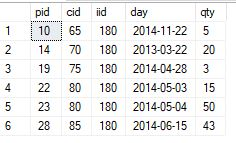
\includegraphics{before.jpg}

\noindent After: the Chocolate Frog purchase records of the customer (cid=80) are deleted.\\

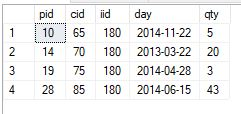
\includegraphics{after.jpg}

\section{Deliverable 6}
Execute:
\begin{verbatim}
delete from item
where iid = 180;
\end{verbatim}

\noindent When we execute the delete command, we get the following error: 
\begin{verbatim}
Msg 547, Level 16, State 0, Line 4
The DELETE statement conflicted with the REFERENCE constraint "FK__purchase__iid__15502E78". 
The conflict occurred in database "CustomerDB_f4a0b", table "dbo.purchase", column 'iid'.
The statement has been terminated.
\end{verbatim}

\noindent This is because the item with iid 180 is referenced by some records in purchase table. If we delete item 180, then the purchase record, which has iid as a foreign key referencing item 180, cannot find the item in the item table, which violates referential integrity. So item 180 cannot be deleted until all the purchase records that reference item 180 are deleted.

\section{Deliverable 7}

Execute:
\begin{verbatim}
update purchase
set qty = 42;
\end{verbatim}

\noindent we update every purchase's quantity to be 42.\\
\\
\noindent capture before recovery: \\
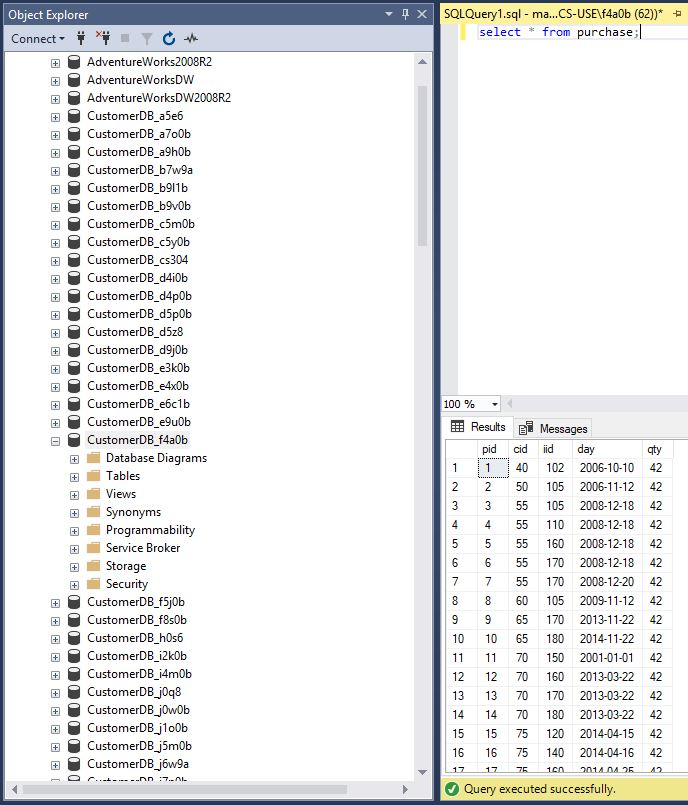
\includegraphics[scale=0.8]{capture_before_recovery}

\section{Deliverable 8}

capture during recovery: \\

\noindent 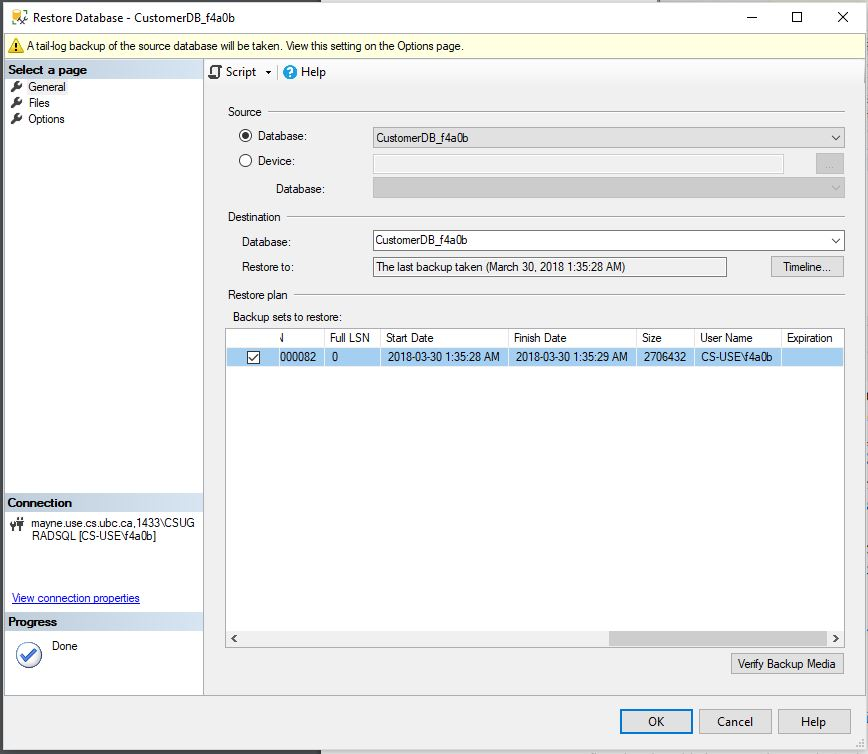
\includegraphics[scale=0.7]{capture_during_recovery}


\section{Deliverable 9}

capture after recovery: \\

\noindent 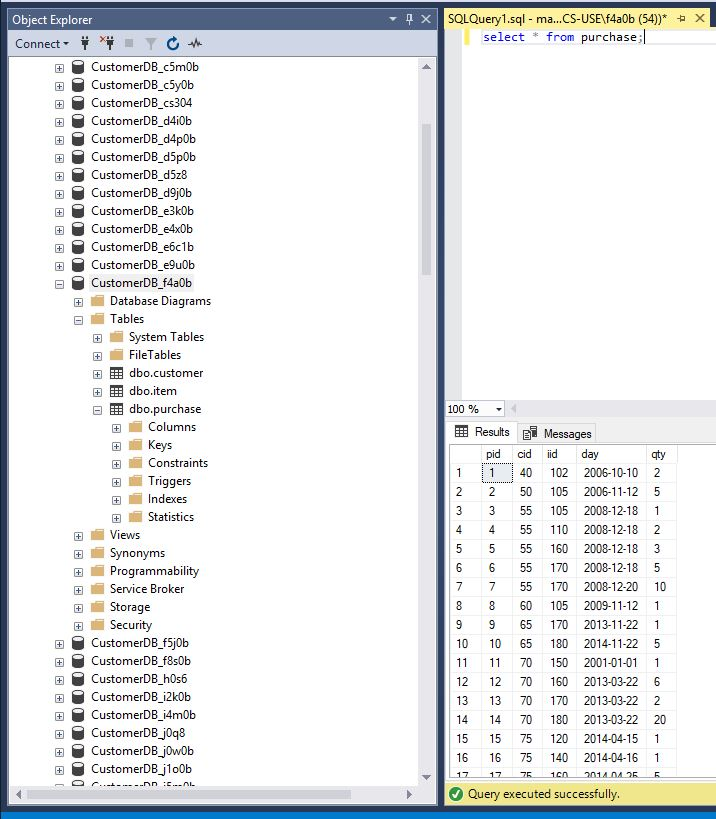
\includegraphics[scale=0.8]{capture_after_recovery}



\end{document}
